Ante los enfoques teóricos y prácticos estudiados anteriormente, nuestro desarrollo de software propio, que permite mostrar de manera gráfica las relaciones entre actores delictuales en el Sistema Penal de la Provincia del Chubut, se potencia como una herramienta vital de apoyo en la toma de decisiones de la investigación penal de bandas delictivas.

Poder visualizar relaciones entre las personas involucradas en casos penales ayuda a los especialistas a detectar triangulaciones, transitividades y por supuesto centralidades en la Red. Todo ello, sumado a los indicios de investigación y la propia expertís en la temática completan una herramienta de análisis para determinar ciertas bandas o grupos altamente relacionados.

En el año 2019 existieron investigaciones vinculadas a reiterados robos de televisores LCD en domicilios, como así también una serie de hechos consecutivos vinculados al robo de cajas fuertes en empresas del parque industrial de la ciudad de Trelew.

La UAC (Unidad de Análisis Criminal), organismo auxiliar de la Procuración General perteneciente al Ministerio Público Fiscal del Chubut, sirvió como equipo de apoyo en la investigación de ambos modus operandi, haciendo uso de toda la información de los legajos fiscales, consultas generales y específicas contenidas en el Sistema Coirón. Fue de vital uso la información referida a los grupos de pertenencia de cada persona, pero devino en un arduo trabajo entrecruzando información de personas, para dar con las supuestas bandas delictivas detrás de estos hechos.

Dichas investigaciones sirvieron como puntapié inicial para realizar este trabajo y poder facilitar la información ya contenida en el sistema de gestión penal, de otra manera, de una forma más directa y visual a la hora de investigar, que sirva directamente como apoyo a la toma de decisiones en las investigaciones de bandas delictivas. 

A continuación se puede observar una visualización extraída de este trabajo, utilizando como filtros de búsqueda dos personas (nodos 116587 y 145262) con muchos casos y relaciones en el sistema, a fin de encontrar si existe algún tipo de relación directa entre ambos, y a su vez si existen nodos que produzcan transitividades o sean a su vez centrales de otros grupos.
Desde la visualización se agregó gracias a la vinculación con el sistema de la oficina de identificación de personas, fotografías para colocar en los nodos y hacer de este trabajo una herramienta aún más potente. Aquellas personas que no hayan sido identificadas en sede judicial no tendrán fotografía. Por cuestiones judiciales se han desenfocado las fotografías y se han colocado identificadores en vez de los nombres reales de las personas intervinientes.
\vspace{-10pt}
\begin{figure}
	\centering
	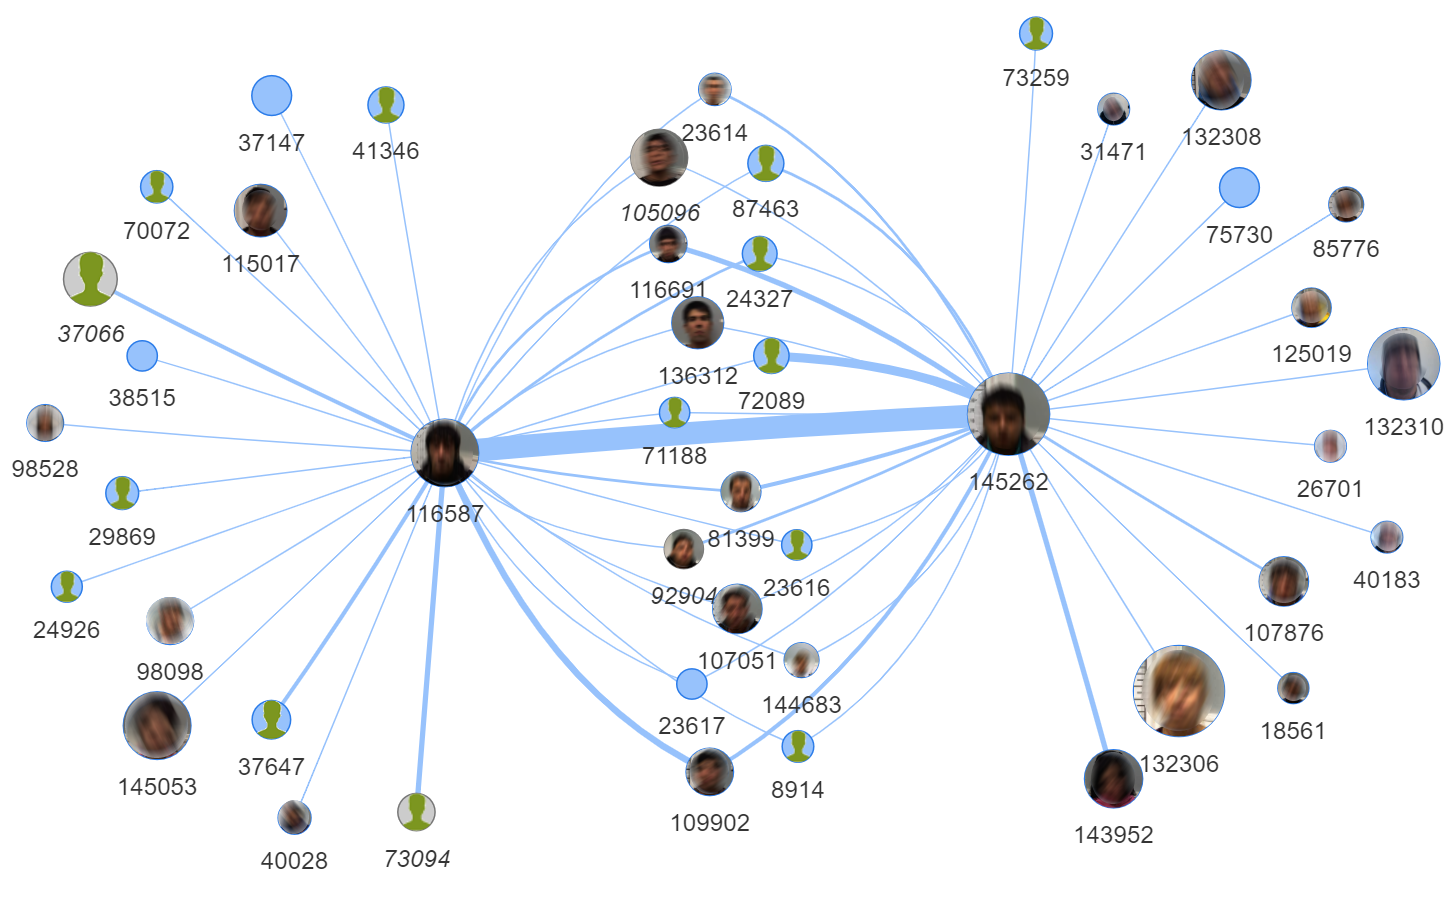
\includegraphics[width=0.75\linewidth]{hermanos-curruman.png}
	\caption{Relación entre dos personas. Se agregan fotografías.} 
	\label{fig:hermanos-curruman}
\end{figure}
\vspace{-10pt}
Como puede verse, existen en la parte central de la imagen muchas personas que se encuentran relacionadas delictualmente con ambos nodos en cuestión. De esta manera se pueden tomar acciones con respecto a estas personas en pos de encontrar patrones de ocurrencia que los vinculen ante la posibilidad de identificarlos como una supuesta banda delictiva. 